
\chapter{Introduction} % enter the name of the chapter here
\label{cha:chapter label} % enter the chapter label here (for cross referencing)


% \section*{Introduction}
Generative Adversarial Networks (GANs) are a powerful deep learning framework introduced by Ian Goodfellow and his colleagues in 2014. They are widely used in generative modeling tasks such as image synthesis, image super-resolution, style transfer, and data augmentation. GANs are unique in their architecture because they consist of two competing neural networks—the Generator and the Discriminator—which are trained simultaneously in an adversarial manner.

\begin{figure}[h!]
    \centering
    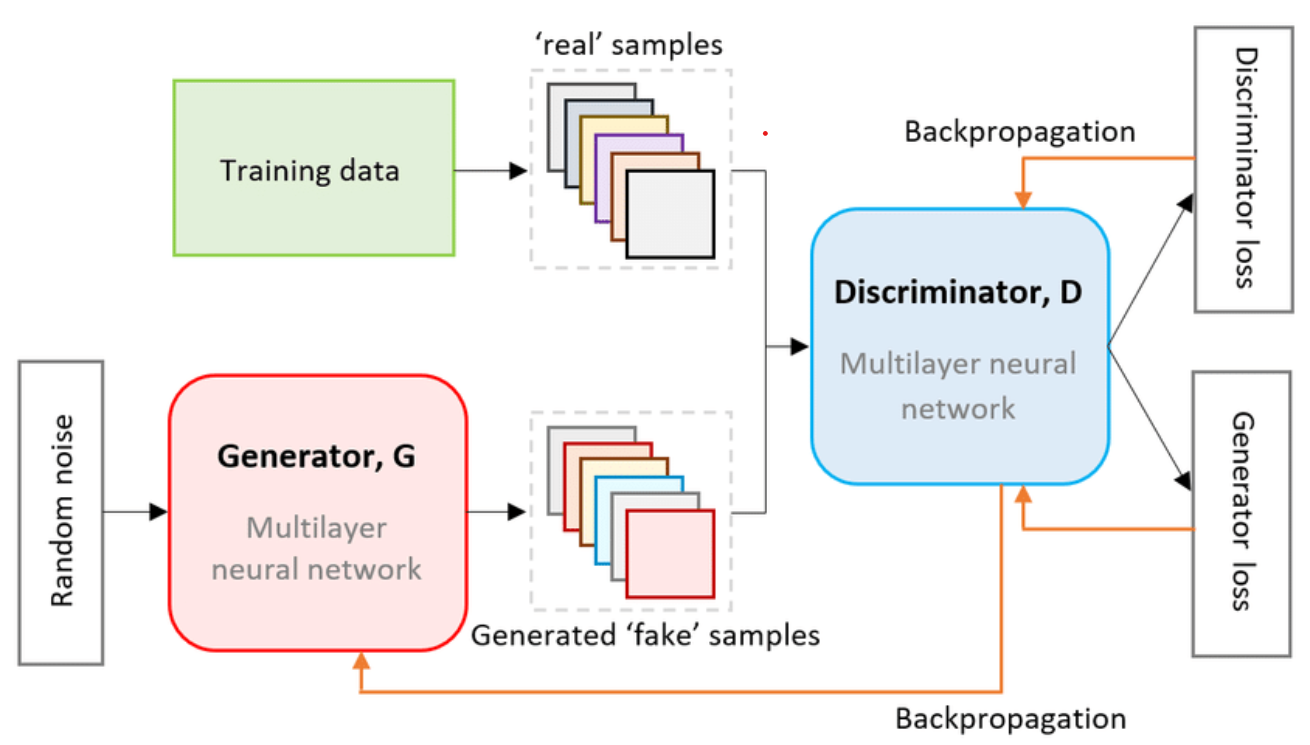
\includegraphics[width=0.7\textwidth]{image/arch.png} % <-- Update with your actual file path
    \caption{GAN Architecture}
    \label{fig:workflow}
\end{figure}
% \subsection*{Components of a GAN}

% A typical Generative Adversarial Network (GAN) consists of two main components:

\begin{itemize}
    \item \textbf{Generator (G):} The generator takes a random noise vector (or a low-resolution image in the case of super-resolution) as input and transforms it into a high-resolution or realistic-looking image. It uses transposed convolution layers or upsampling layers to increase the spatial dimensions of the image and is trained to produce outputs that look as real as possible to the discriminator.
    
    \item \textbf{Discriminator (D):} The discriminator is a binary classifier that takes an image as input and outputs the probability of whether the image is real (from the dataset) or fake (generated by the generator). It uses convolutional layers to extract features and is trained to correctly classify the images.
\end{itemize}

Both the generator and discriminator are trained simultaneously using a minimax loss function:

\begin{equation}
    \min_G \max_D \; \mathbb{E}_{x \sim p_{\text{data}}(x)} [\log D(x)] + \mathbb{E}_{z \sim p_z(z)} [\log(1 - D(G(z)))]
\end{equation}

Here:
\begin{itemize}
    \item $x$ is a real data sample from the true data distribution $p_{\text{data}}$.
    \item $z$ is a noise vector sampled from a prior distribution $p_z$ (e.g., uniform or Gaussian).
    \item $G(z)$ is the image generated by the generator from noise $z$.
    \item $D(x)$ is the probability output by the discriminator that $x$ is a real image.
\end{itemize}
\vspace{0.07cm}
\textbf{Convolutional Neural Networks (CNNs):}\\
Convolutional Neural Networks (CNNs) are a class of deep learning models particularly well-suited for image processing tasks. They use convolutional layers to automatically learn spatial hierarchies of features from input images. CNNs are effective at tasks like image classification and object detection, but in image super-resolution, they often produce blurry results due to their reliance on pixel-wise losses. Unlike GANs, CNNs lack the ability to generate high-frequency details and perceptual realism.


% \section{Objective:}
% \begin{itemize}
%     \item To study and implement GANs for enhancing image resolution.
  

% \item To develop a technique that transforms low-resolution images into high
% resolution outputs.

% \item To evaluate the performance of the model on datasets relevant to medical
%  imaging, streaming, and security.
% \end{itemize} 

\section{Problem statement}
The aim of this project is to address the challenge of generating high-resolution images from low-resolution inputs using a deep learning approach. Specifically, the project seeks to implement and evaluate the Enhanced Super-Resolution Generative Adversarial Network (ESRGAN) to reconstruct visually pleasing and high-quality images, thereby overcoming the limitations of conventional interpolation methods.

% \section{What is the problem}
% In many practical applications like satellite imaging, medical diagnostics, video surveillance, and old photo restoration, the available images are often of low quality or resolution. Traditional image upscaling techniques such as bicubic interpolation often result in blurry or pixelated images with loss of texture and fine details. The problem is to create a system that can enhance image resolution while preserving fine textures, edges, and realistic details, thus improving the overall visual quality.

\section{Why is this a project related to this class}
This project relates directly to the subjects of Machine Learning, Deep Learning, and Computer Vision, which are essential components of the curriculum in Computer Science and Engineering(AI\&ML). It involves the use of Neural Networks, Generative Adversarial Networks (GANs), image processing, and data-driven model training, which align with the theoretical and practical knowledge imparted in these courses. The project also builds hands-on experience with frameworks like PyTorch or TensorFlow, strengthening both academic and industry-ready skills.

\section{Area or Scope of Investigation}
\begin{itemize}
    % \item Domain: Deep Learning, Computer Vision, Image Processing
    
    % \item Tools \& Technologies: Python, PyTorch, Matplotlib, PIL, ESRGAN architecture
    
    % \item Dataset Used: DIV2K (high-resolution image dataset used for super-resolution tasks)
    
    % \item Scope:
    % \begin{itemize}
        \item Training ESRGAN on real-world image datasets.
        \item Understanding the internal architecture of GANs and their applications.
        \item Visualizing and analyzing the results using graphs and image comparisons.
        \item Enhancing the project to real-time applications such as video upscaling or photo enhancement tools in the future.
    % \end{itemize}
\end{itemize}
